\chapter{Introduction to Software Design}

\section{Complexity}
Complexity is anything related to the structure of a software system that makes
it hard to understand and modify the system.

\begin{equation*}
  \centering
  C = \sum_p c_pt_p
\end{equation*}

Where $C$ is determined by all software parts $p$, $c_p$ is the complexity of part $p$,
and $t_p$ is the fraction of time spent on part $p$.

\subsection{Syntax complexity}

\begin{itemize}
  \item Change amplification: change require operating in different places
  \item Cognitive load: how mutch information to learn to understand and perform a task. Some times is better to write longer code to reduce the complexity and so the cognitive load.
  \item Unknown unknowns: there are partes of the system that we don't know where they are or even that they exist.
\end{itemize}

\subsection{Cause of complexity}

\textbf{Dependency}: When we need to understand or modify a part of the code, we need to understand or modify other parts of the code. Try to reduce the number of dependencies and the complexity of the dependencies.

\textbf{Obscuiry}: alla the important information shoul be clearly visible.

\subsection{Strategical vs. Tactical Programming}

\begin{itemize}
  \item \textbf{Tactical programming}: focus on having code that works as fast as possible. "Move fast and break things".
  \item \textbf{Strategical programming}: focus on long term maintainability and scalability. "Working code is not enough".
\end{itemize}

\section{Modules}

To improve and eliminate dependency and complexity, we can use modules. A module is a part of the code that has a well defined interface and a well defined implementation.

\begin{itemize}
  \item \textbf{Interface}: what we need to know to use the module. Formal part, possible checked by the compiler. Represents a cost.
  \item \textbf{Implementation}: how the module works. Ideall much more complex than the interface. Represents a benefit.
\end{itemize}

\subsection{Abstraction}

What we tipically do is to perform an abstraction. Abstraction means selective removal of information.
Is a simplified view of the something that omits "unimportant" information. Omitting information can lead to eads to unknowns and
keeping unimportant information can leads to cognitive overload.

\subsubsection{Deep modules and shallow interfaces}


\begin{minipage}{0.95\linewidth}
  % Primo blocco: 50% dello spazio per il codice
  \begin{minipage}{0.65\linewidth}

    \textbf{Deep modules}: modules with a simple interface and a complex implementation. They are good because they reduce the cognitive load and the change amplification. They are bad because they can lead to unknown unknowns.
    \newline\textbf{Shallow interfaces}: modules with a complex interface and a simple implementation. They are good because they reduce the unknown unknowns. They are bad because they can lead to cognitive overload and change amplification.


  \end{minipage}% <-- IMPORTANTE: il simbolo % qui evita spazi bianchi extra
  \hfill
  \begin{minipage}{0.3\linewidth}

    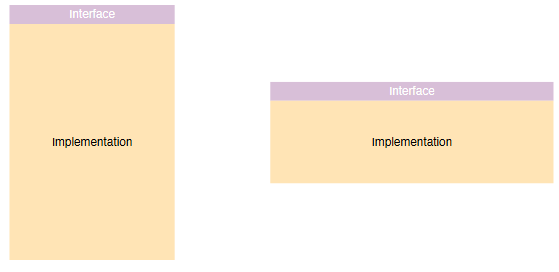
\includegraphics[width=1\linewidth]{images/DI-esempio1.png}

  \end{minipage}
\end{minipage}





\begin{flushleft}
  \begin{minipage}[t]{0.45\linewidth}
    \raggedright
    \subsection{Information Hiding}
    Information hiding is the principle of hiding the implementation details of a module from the users of the module.
    Example sort function: we want to sort a list of numbers, we don't care about how the sorting algorithm used.
  \end{minipage}%
  \hfill
  \begin{minipage}[t]{0.45\linewidth}
    \raggedright
    \subsection{Information Leakage}

    Is the opposite of information hiding. Occurs when the implementation details of a module is reflected
    in multiple modules with consequences of creating dependencies.
  \end{minipage}
\end{flushleft}



\subsection{Information Hiding Red Flags}
\begin{itemize}
  \item \textbf{temporal decomposition}: execution order is reflected in the code structure. Operations that happen
        in different times are in different classes.
  \item \textbf{overexposure}: API forces knowledge about rarely used features to use common ones.
        E.g. \mintinline{java}{BufferedReader r = new BufferedReader(new InputStreamReader(System.in));}
  \item \textbf{Too many classes}: code is divide into too many shallow classes.
\end{itemize}

\subsection{Method separation}
Better together or Better apart?

\begin{itemize}
  \item \textbf{Bring together}: if information is shared, if we simplify the interface, if we eliminate duplication.
  \item \textbf{Separate}: if the code is general purpose or specific purpose.
\end{itemize}

\subsubsection{Method separation red flags}

If we have a lot of repeded code and/or we mixed specific and general code, means we have put together code that should be separated.


\subsection{Do one simple thing and complexity}

\begin{center}
  \centering

  \begin{minipage}{1\linewidth}
    % Primo blocco: 50% dello spazio per il codice
    \begin{minipage}{0.5\linewidth}

      Each method should do one thing and do it completely

    \end{minipage}% <-- IMPORTANTE: il simbolo % qui evita spazi bianchi extra
    \hfill
    \begin{minipage}{0.45\linewidth}

      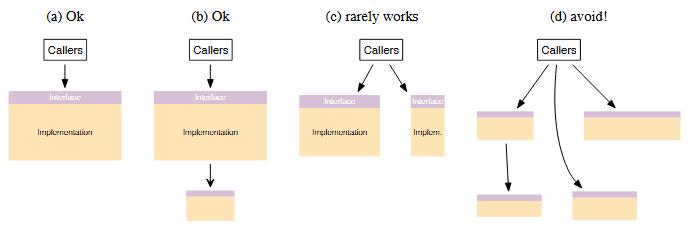
\includegraphics[width=1\linewidth]{images/DI-esempio2.png}

    \end{minipage}
  \end{minipage}
\end{center}



\section{Obscurity}

Obscurity is the principle of making the important information clearly visible and the unimportant information hidden.
Obscurity is a great source of complexity. Obscure code is hard to Understand and creates more Bugs.

The solution to obscurity is writing obvious code, this means with a quick glance we can understand what the code does.
We can achieve this by using abstraction layers.


\subsection{Abstraction layers}

Software systems are composed in layers. Higher layers use the facilities provided by lower layers.

Abstraction simplifies understanding and reduces obscurity.

In a well-designed system, each layer provides a different abstraction from the layers above and below it.


\subsubsection{Abstraction Layers Red Flags}

Some red flags that indicate that we have a problem with abstraction layers are:

\begin{itemize}
  \item \textbf{Pass-Through methods}: is a method that does nothing but call another method.
  \item \textbf{Pass-Through variables}: is a variable that is passed through over and over down a long chain of method calls.
\end{itemize}

\subsection{Writing Comments}

Another method to reduce obscurity is writing comments. If users need to read a method code to use it, there is no
abstraction.

Comments should describe things that are not obvious in
the code:

\begin{itemize}
  \item \textbf{Pick conventions}: write comments like other persons in the project
  \item \textbf{Don't repeat code}: avoid redundant comments that simply restate what the code already makes clear
  \item \textbf{Higher level comments enhance intuition}
  \item \textbf{Delayed comments are bad comments}
  \item \textbf{Use comments as design tool}
\end{itemize}


\subsection{Naming}
Toghether with comments, naming is a great tool to reduce obscurity. Bad names cause bugs.
Name should create a image in mind of the reader about the nature of the thing being named.
Names should be precise and consistent.

\section{Errors and Anomalies}
Exceptions add complexity because they create dependencies between the code and if they are easy
to throw they are hard to handle.

A piece of code might throw exceptions in different ways:

\begin{itemize}
  \item Caller may provide bad arguments or configuration
  \item Invoked method may not able to complete the request
  \item In distributed systems network packets may be lost or delay or peers may communicate in unxpected ways
  \item The code may detect bugs or internal inconsistencies or situations that are not prepared to handle
\end{itemize}

\subsection{Define Errors out of Existence}
What are the solutions to errors? Define errors out of existence.
This means, not ignore the error but to redefine the behavior of a method so that no error is
required.

E.g. \mintinline{java}{String.substring(int beginIndex, int endIndex)} it throws different exceptions Some in only specific cases.
This is completly avoidable and unnecessary.


\subsection{Limit exceptions}
There are some methods to limit the number of exceptions that a method can throw:

\begin{itemize}
  \item Handle exceptions at the point where they are thrown, if possible
  \item Exception aggregation means handle different exceptions with same handler
  \item Just crash
  \item Mask exceptions avoiding unexpected exceptions
\end{itemize}


\section{Dependency Dimensions}

% \begin{enumerate}
%   \item Structural (Code-Level) Dependencies
%   \item Runtime / Distribution Dependencies
%   \item Data-Level Dependencies
%   \item Behavioral Dependencies
% \end{enumerate}

\subsection{Structural (Code-Level) Dependencies}

\begin{itemize}
  \item \textbf{Implementation Dependency}: some piece of code depends on a concrete class instead of an abstraction
  \item \textbf{Construction Dependency}: you depend on how a collaboration, another class, is created.
  \item \textbf{Compile-Time Dependency}: the module knows something at compile time
\end{itemize}

\subsection{Runtime / Distribution Dependencies}

Often linked to distributed architectures.

\begin{itemize}
  \item \textbf{Spatial Dependency}: A component depends on the location of another component. E.g. hard-coded URLs
  \item \textbf{Temporal Dependency}: A component depends on another being available at the same time. E.g. remote method calls or servers
  \item \textbf{Synchronization Dependency}: A component depends on another to complete work before continuing. E.g.  synchronous request/response
\end{itemize}

\subsection{Data-Level Dependencies}
\begin{itemize}
  \item \textbf{Data Dependency}: One component depends on another’s internal data model. E.g. shared database
  \item \textbf{Schema Dependency}: Multiple services depend on the same database schema or representation structure. E.g. DB schema, XML/Json schema
\end{itemize}

\subsection{Behavioral Dependencies}
\begin{itemize}
  \item \textbf{Control Flow Dependency}: One component dictates another's execution path. E.g. Centralized process managers
  \item \textbf{Transactional Dependency}: E.g. Components rely on atomic distributed consistency.
  \item \textbf{Timing Assumption Dependency}: Assumptions about response time or ordering. E.g. "Service must respond in <50ms" or Event ordering assumptions
\end{itemize}

